\documentclass[11pt]{scrartcl}
\usepackage[a4paper]{geometry}

\usepackage{graphicx}
%\graphicspath{ {./images/} }

\usepackage{fancyhdr}
\pagestyle{fancy}
\fancyhf{}
\fancyhead[L]{SPIROMETRIE} %Kopfzeile links
\fancyfoot[C]{\thepage}

\usepackage[utf8]{inputenc}
\usepackage{csquotes}
\usepackage[german]{babel}

\usepackage{setspace}

\usepackage{caption}
\usepackage{float}

\usepackage{hyperref}
\usepackage{pdfpages}

\hypersetup{
    pdftitle = {Spirometrie},
    pdfsubject = {Biomedizinischesystemtechnik Praktikum},
    pdfauthor = {Leona K{\"o}ck, Chris R{\"u}ttimann},
    pdfkeywords = {} ,
    pdfcreator = {pdflatex},
    pdfproducer = {LaTeX with hyperref}
}

\usepackage[
    style=apa,
    backend=biber,
    sortcites=false,
    sorting=none,
    hyperref=true,
    backref=false
]{biblatex}
\usepackage{amsmath}
\usepackage[T1]{fontenc}
\usepackage{siunitx}
\addbibresource{Quellen.bib}

\begin{document}
    \pagenumbering{Alph}
% ---------------------
% Titlepage
% ---------------------
    \begin{titlepage}
        \begin{center}
        {\LARGE OST Ostschweizer Fachhochschule}
            \\[1.5cm]
            \linespread{1.2}\large { Biomedizinischesystemtechnik Praktikum }

            \huge{\bfseries Spirometrie}
            \\%[1.5cm]
            \large{durchgef{\"u}hrt am 22. März 2021}
            \\[1.5cm]
   %         \linespread{1}
           
\includegraphics[width=8cm]{../images/ost_logo.eps}
           \\[1cm]
            {\small{Autoren}}\\
            {\Large{Leona K{\"o}ck}}\\
            {\Large{Chris R{\"u}ttimann}}
            \\[1cm]

            \vspace*{\fill}
            \large{\today}
        \end{center}

    \end{titlepage}

% ---------------------
% Abstract
% ---------------------
    \pagenumbering{Roman}
 %   \pdfbookmark[section]{Abstract}{abstract}
 %   \section*{Abstract}
    \addtocounter{section}{0}

 %   \pagebreak
    \setstretch{1.25}
% ---------------------
% Table of contents
% ---------------------
    \tableofcontents
    \pagebreak


% ---------------------
% Body
% ---------------------
    \pagenumbering{arabic}

    \section{Problemlösung}

    \subsection{Vorbereitung}

    Zur Vorbereitung wurden mithilfe der Praktikumsanleitung~\parencite{Spirometrie} die folgenden Fragen beantwortet: %todo

    \begin{itemize}
        \item[a] Schätzen Sie den Einfluss des barometrischen Luftdruckes zwischen 0m (Meereshöhe, 101 kPa) und 2000m (79 kPa) ab!
                 Der Wasserdampfdruck betrage in beiden Fällen bei 20°C und 40\% Luftfeuchtigkeit 0.9kPa.
        \item[]  $V_{BTPS}=V_{ATP}*\frac{273.2+37}{273.2+t}*\frac{P_B-P_{H_2Ot}}{P_B-6.266}$
        \item[] $t$: Umgebuntstemperatur in °C
        \item[] $P_B$: Barometerdruck in kPa
        \item[] $P_{H_20t}$: Wasserdampfdruck bei Umgebungstemperatur $t$
        \item[] Meereshöhe: $\frac{273.2+37}{273.2+20}*\frac{101-0.9}{101-6.266}=1.118$
        \item[] 2000m : $\frac{273.2+37}{273.2+20}*\frac{79-0.9}{79-6.266}=1.136$
        \item[] Der Einfluss beträgt ca. 1.5\%
        \item[b] Wie gross ist der Einfluss der Umgebungstemperatur bei 10°, 20° und 30° C auf Meereshöhe?
        \item[] 10° C: $\frac{273.2+37}{273.2+10}*\frac{101-0.9}{101-6.266}=1.157$
        \item[] 20° C: $\frac{273.2+37}{273.2+20}*\frac{101-0.9}{101-6.266}=1.118$
        \item[] 30° C: $\frac{273.2+37}{273.2+30}*\frac{101-0.9}{101-6.266}=1.081$

    \end{itemize}

    \subsection{Messung}

    Für die Messungen wurden folgende Materialien benötigt:

    \begin{itemize}
        \item PC mit Spirometrieprogramm (EasyOne connect)
        \item Messgerät (Easy on-PC von ndd, SN-202878)
    \end{itemize}

    Das Messgerät ist ein offenes System, bei dem in die freie Atmosphäre geatmet wird.
    Jeder Proband verwendete eine eigene Spirette.

    \section{Ergebnisse}
    \subsection{Proband Chris Rüttimann}

    \begin{figure}[H]
        \centering
        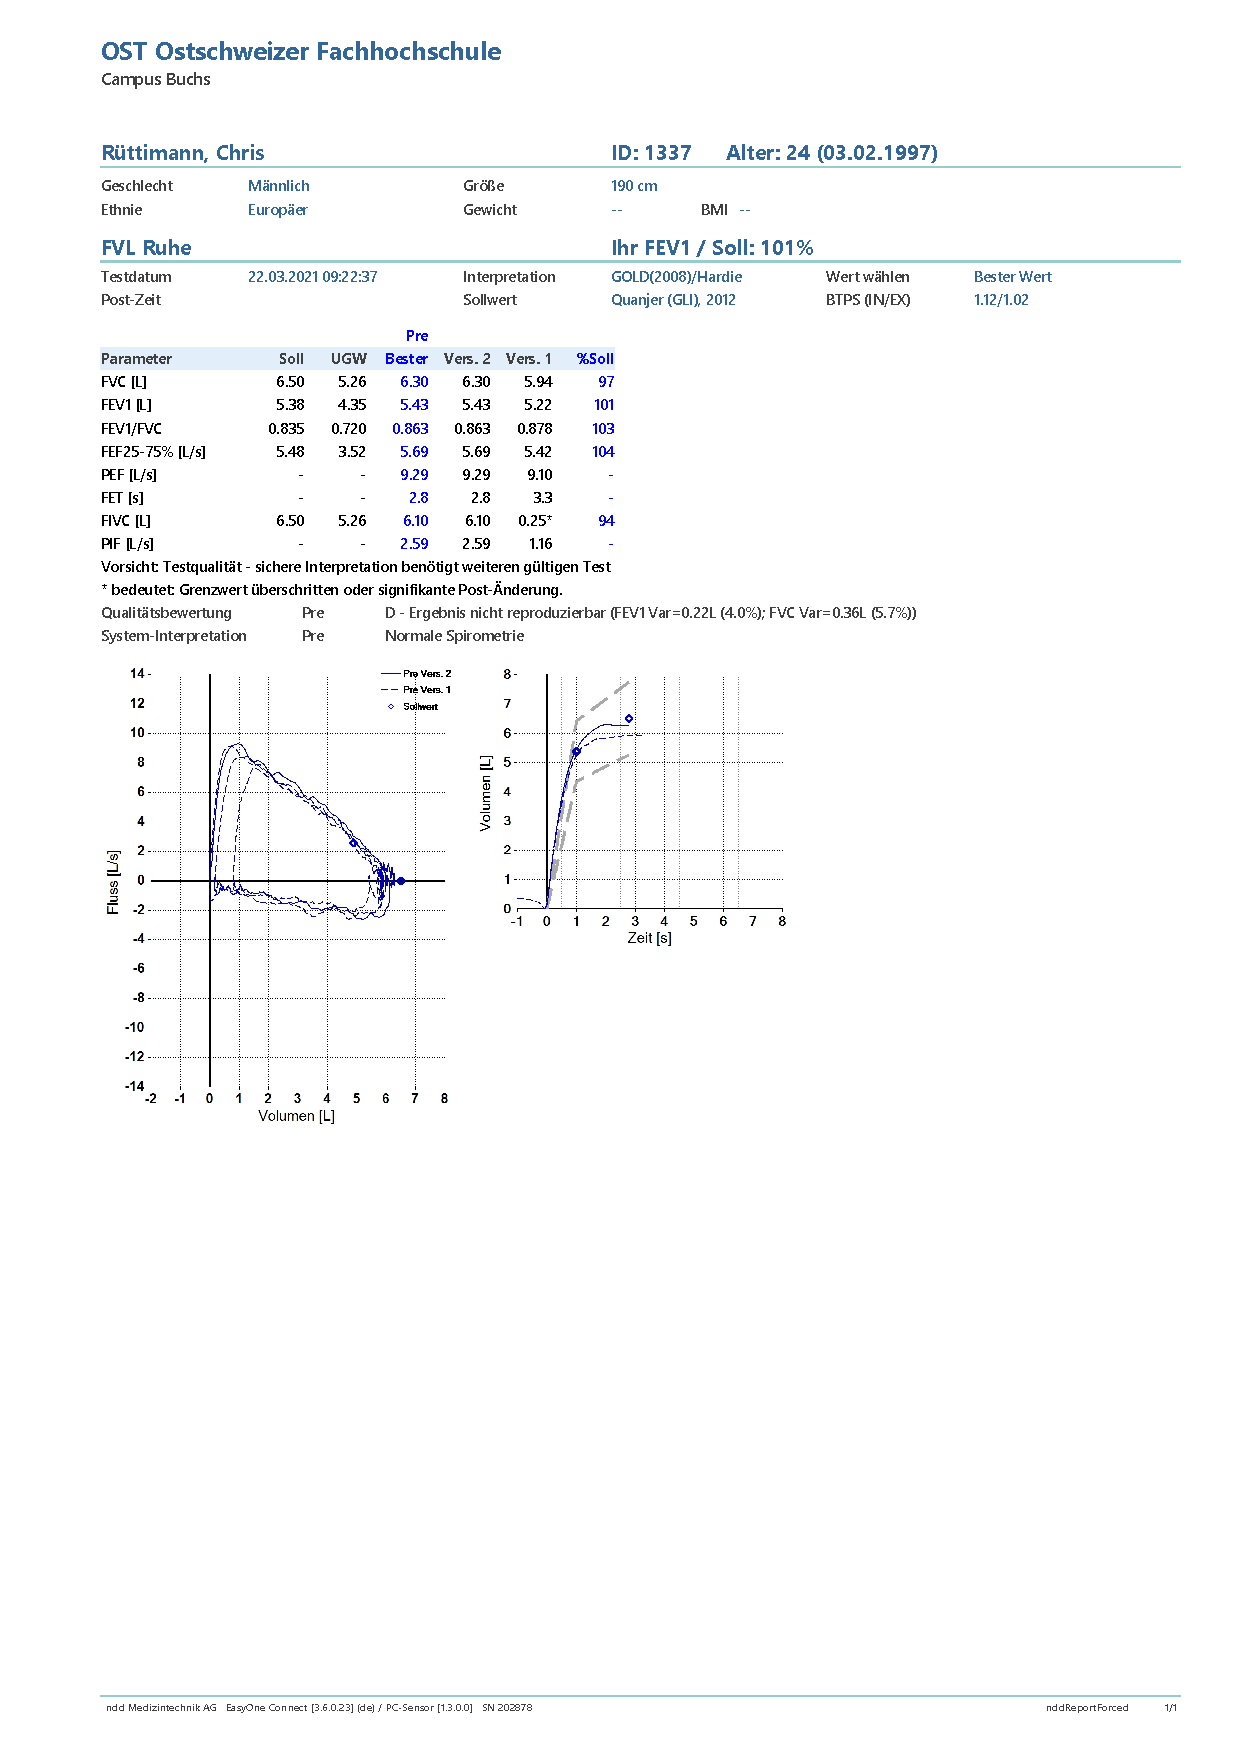
\includegraphics[clip, trim=1cm 10cm 0cm 11cm, width=15cm]{Dateien/Chris1.pdf}
        \caption{Chris, Messreihe 1}
    \end{figure}

    \begin{figure}[H]
        \centering
        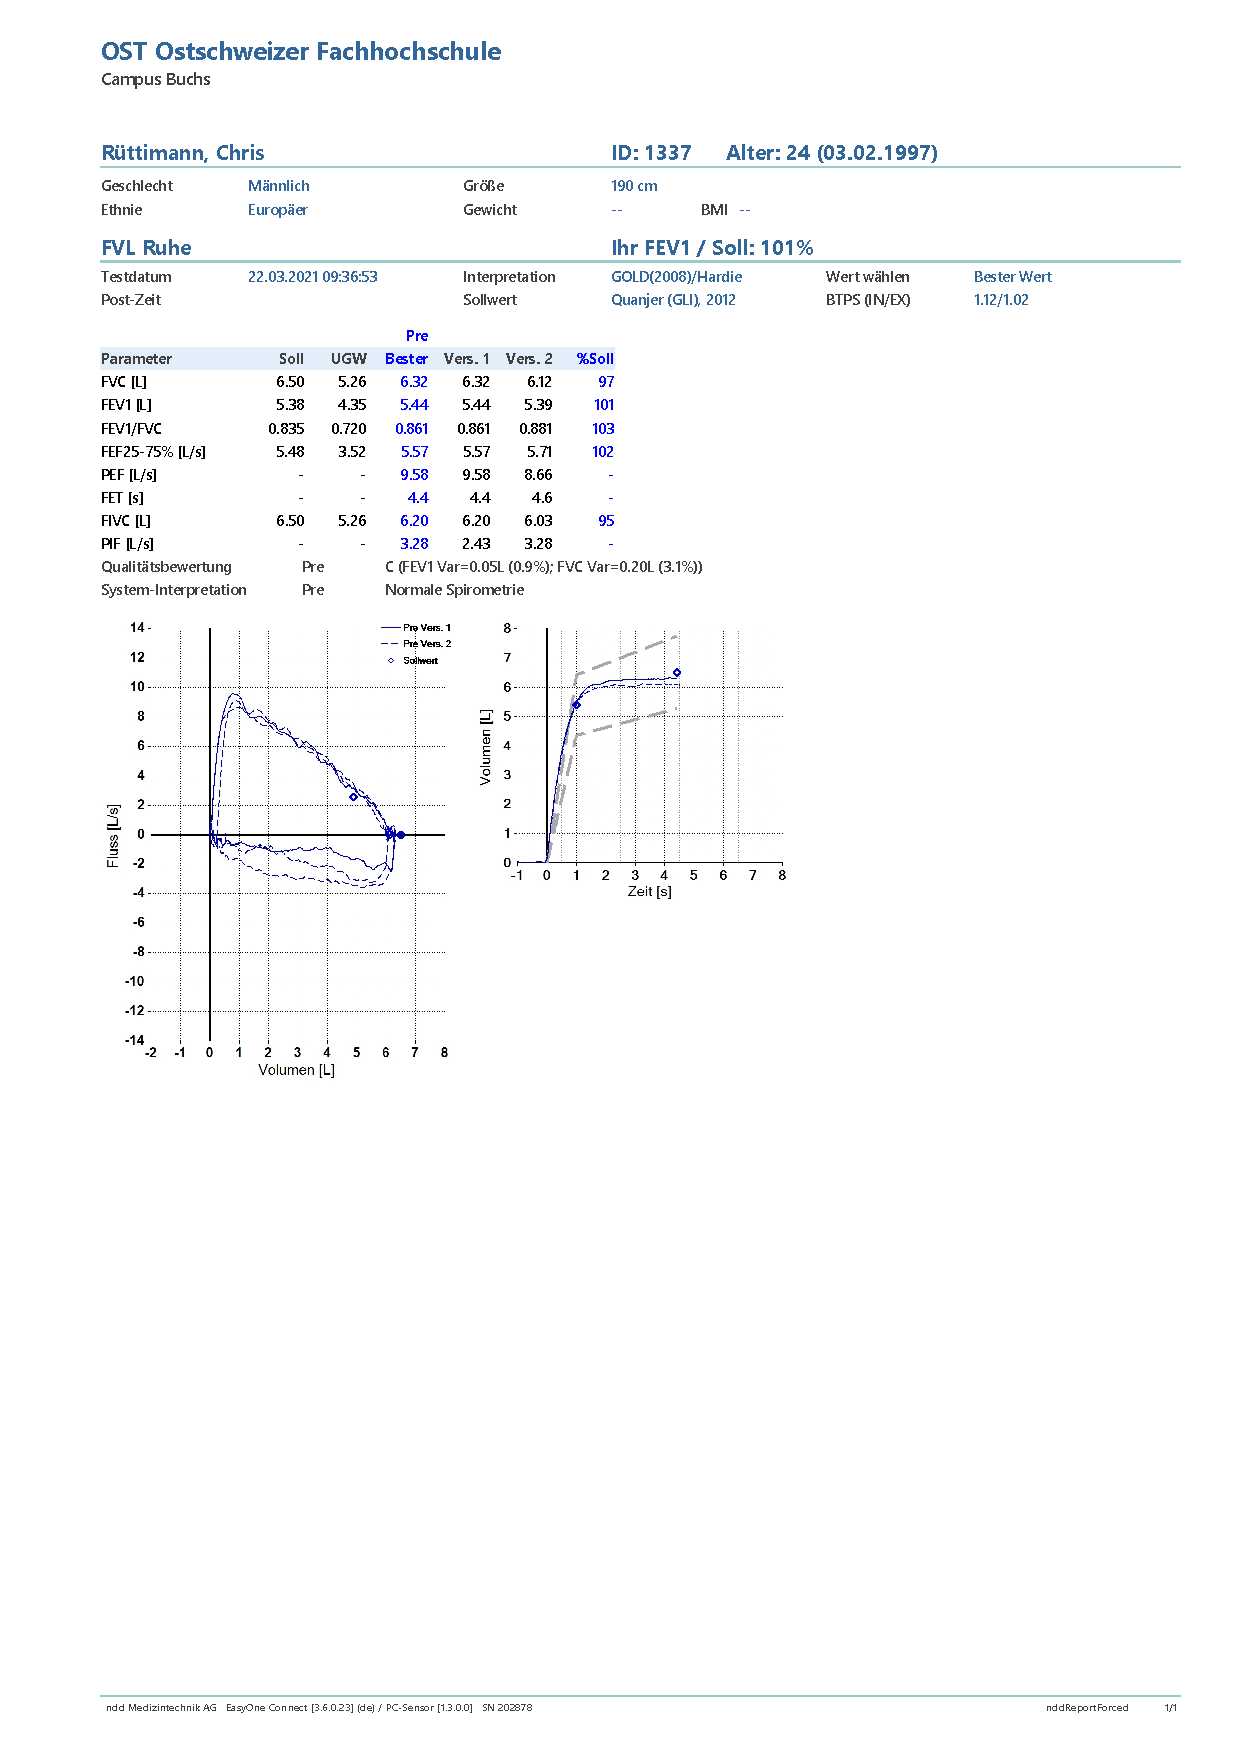
\includegraphics[clip, trim=1cm 10cm 0cm 11cm, width=15cm]{Dateien/Chris2.pdf}
        \caption{Chris, Messreihe 2}
    \end{figure}

    Die Messungen zeigen, dass bei Proband Chris die Lungenfunktion dem erwarteten Wert entsprechen.
    Es können keine Abweichungen festgestellt werden, die auf eine Lungenkrankheit deuten.

    \pagebreak

    \subsection{Probandin Leona Köck}

    \begin{figure}[H]
        \centering
        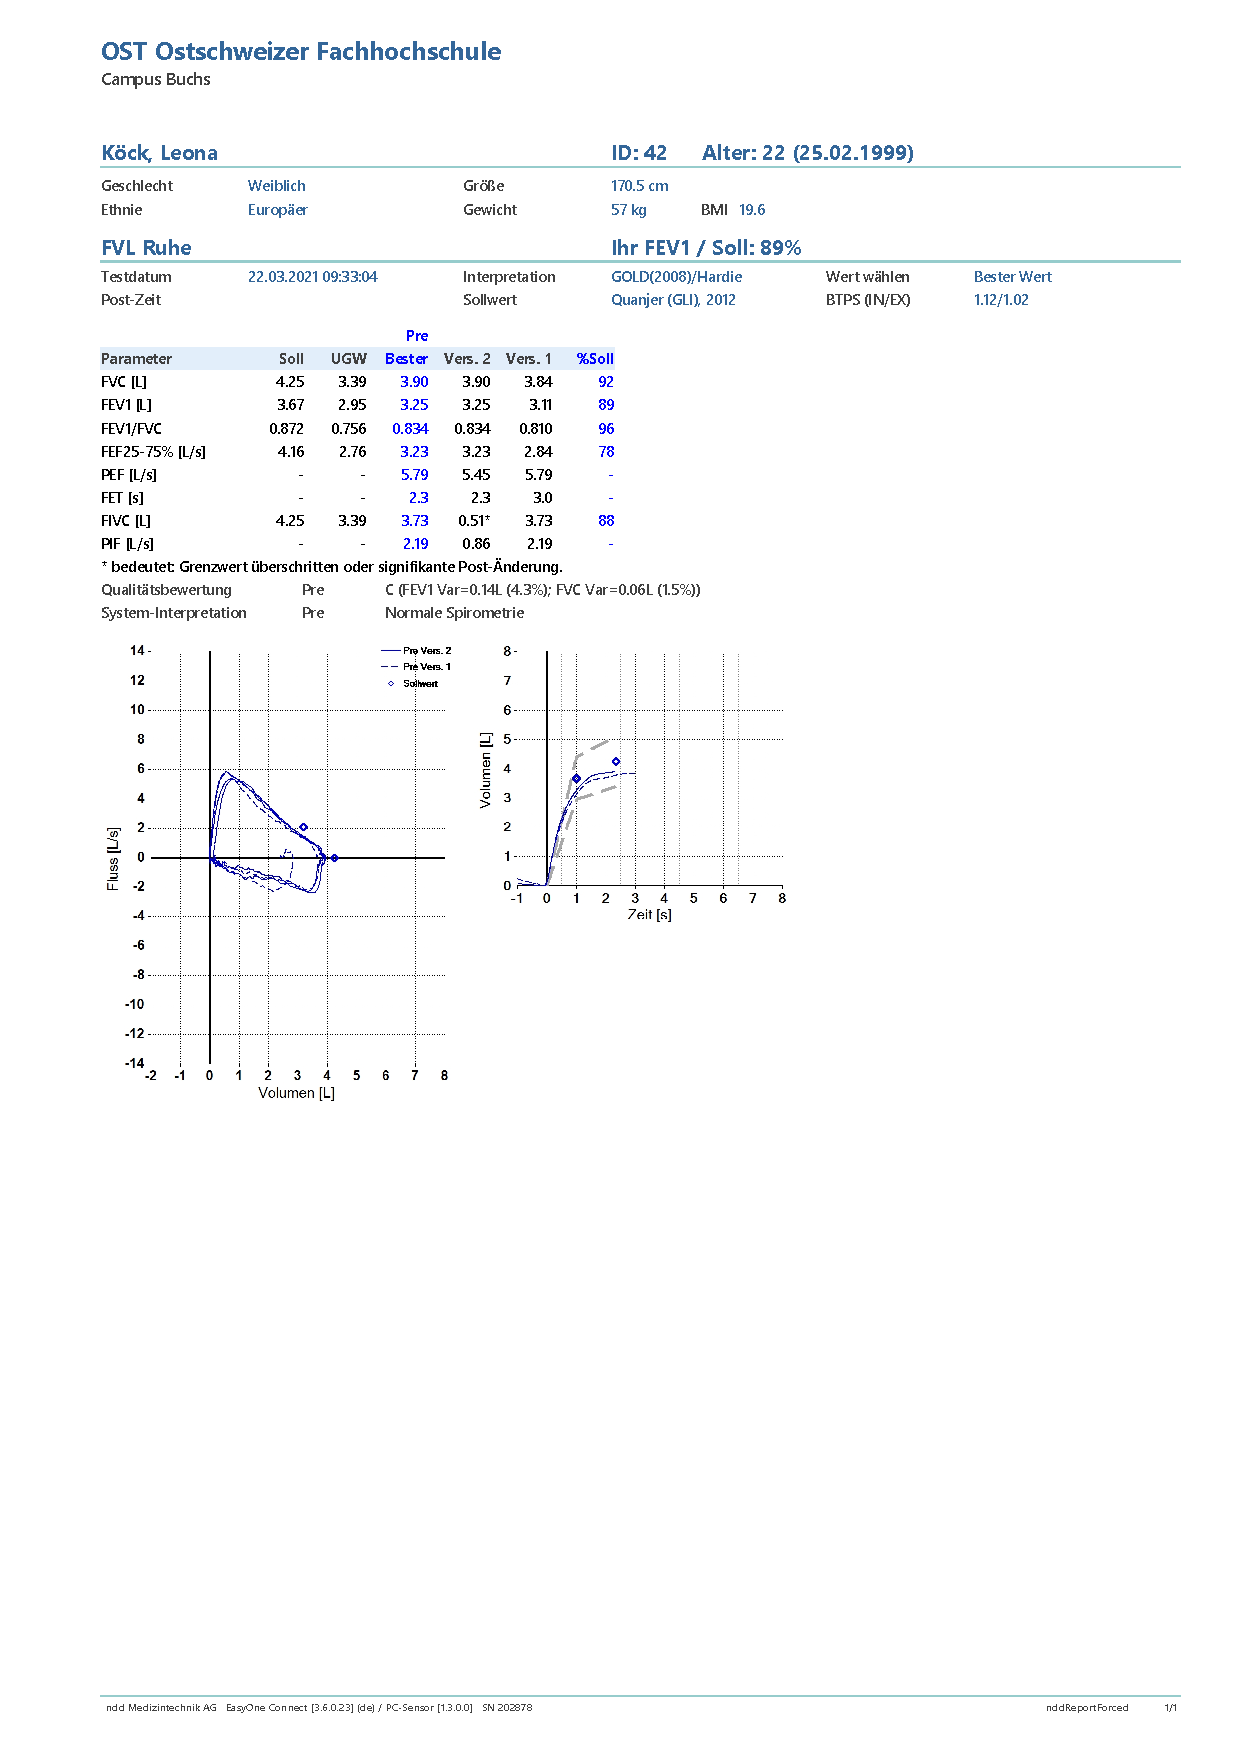
\includegraphics[clip, trim=1cm 10cm 0cm 10.6cm, width=15cm]{Dateien/Leona1.pdf}
        \caption{Leona, Messreihe 1}
    \end{figure}

        \begin{figure}[H]
        \centering
        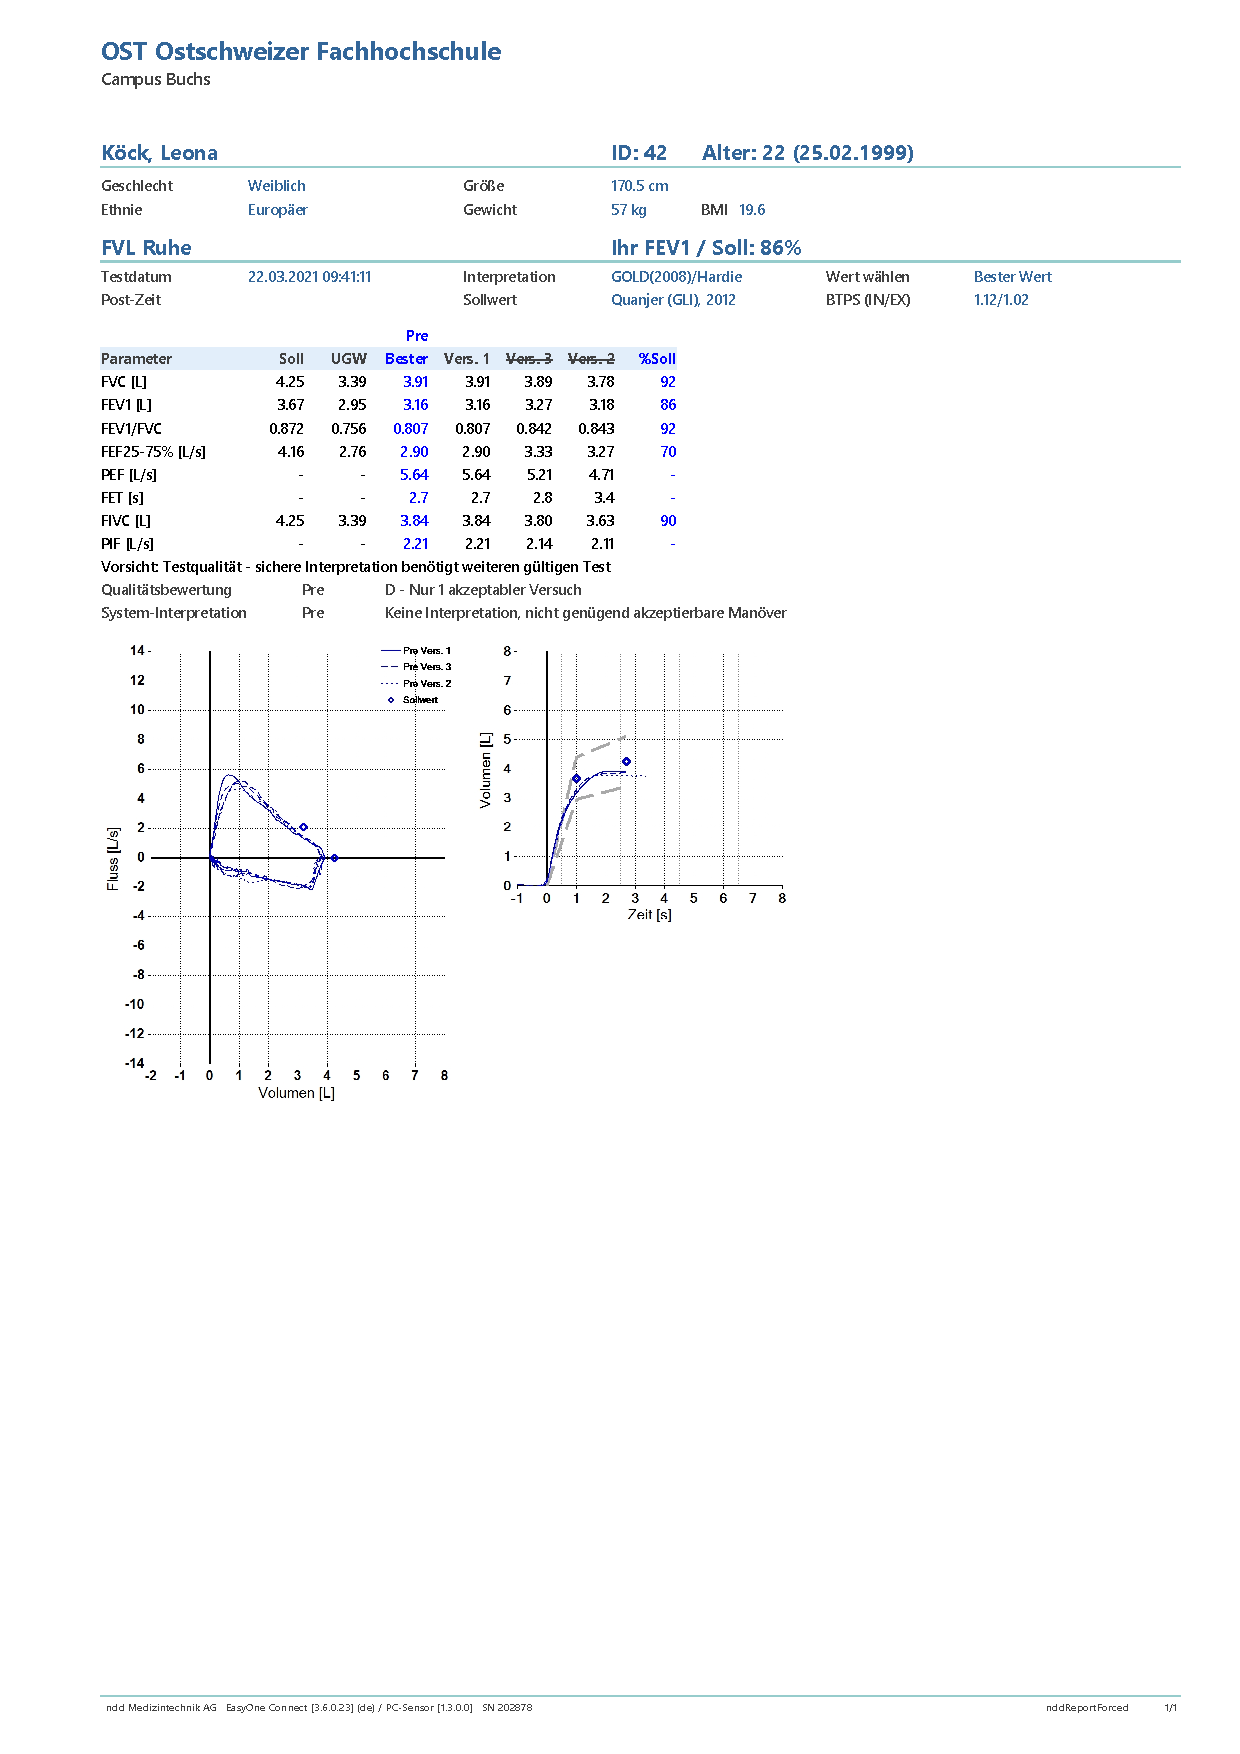
\includegraphics[clip, trim=1cm 10cm 0cm 10.6cm, width=15cm]{Dateien/Leona2.pdf}
        \caption{Leona, Messreihe 2}
        \end{figure}

    Bei Probandin Leona ist eine sehr leichte Obstruktion erkennbar.
    Es ist bekannt, dass ihr linker Lungenflügel etwas kleiner ist wie im Durchschnitt.

    \section{Lungenkrankheiten}

    \begin{figure}[H]
        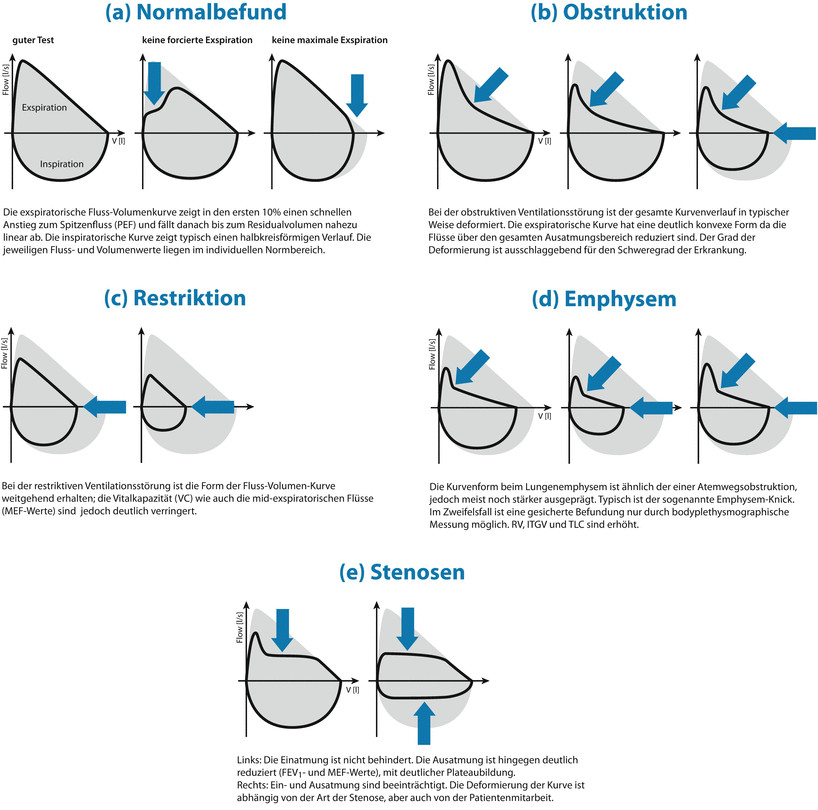
\includegraphics[width=15cm]{Dateien/Flusskurve.jpeg}
        \caption{Fluss-Volumenkurven, \cite{Flusskurven}}
        \label{fig:flusskurve}
    \end{figure}

    Abbildung \ref{fig:flusskurve} zeigt verschiedene Fluss-Volumenkurve und die dazugehörigen medizineschen Befunde.
    Bei einer Obstruktion ist die Kurve konvex deformiert.
    Liegt eine Restriktion vor, hat die Kurve dieselbe Form wie beim Normalbefund, ist aber kleiner.

    \pagebreak

    \section*{Eigenständigkeitserklärung}
    \addcontentsline{toc}{section}{Eigenständigkeitserklärung}

    Hiermit bestätigen wir, dass wir diesen Bericht selbstständig und ohne fremde Hilfe verfasst haben.
    Alle verwendeten Quellen wurden entsprechend dem APA-Standard gekennzeichnet.
    \\[3cm]


    \begin{figure}[H]
        
\includegraphics[width=4cm]{.././images/Unterschrift_Leona.png}
    \end{figure}
    \begin{tabular}{@{} l@{}}
        \hline \\
        \makebox[6cm]{Leona Köck}\\[2cm]
    \end{tabular}


    \begin{figure}[H]
        
\includegraphics[width=4cm]{.././images/Unterschrift_Chris.png}
    \end{figure}
    \begin{tabular}{@{} l@{}}
        \hline\\
        \makebox[6cm]{Chris Rüttimann}
    \end{tabular}

    \pagebreak
% ---------------------
% References
% ---------------------
    \printbibliography
    \addcontentsline{toc}{section}{Literaturverzeichnis}

% ---------------------
% List of figures
% ---------------------
%    \listoffigures
%    \addcontentsline{toc}{section}{Abbildungsverzeichnis}
%    \pagebreak

% ---------------------
% List of tables
% ---------------------
%\listoftables

% ---------------------
% Anhang
% ---------------------

\appendix

    \section{Messung 1 Chris}
    \label{sec:chris1}

    \begin{figure}[H]
        \hspace*{-3cm}
        \centering
        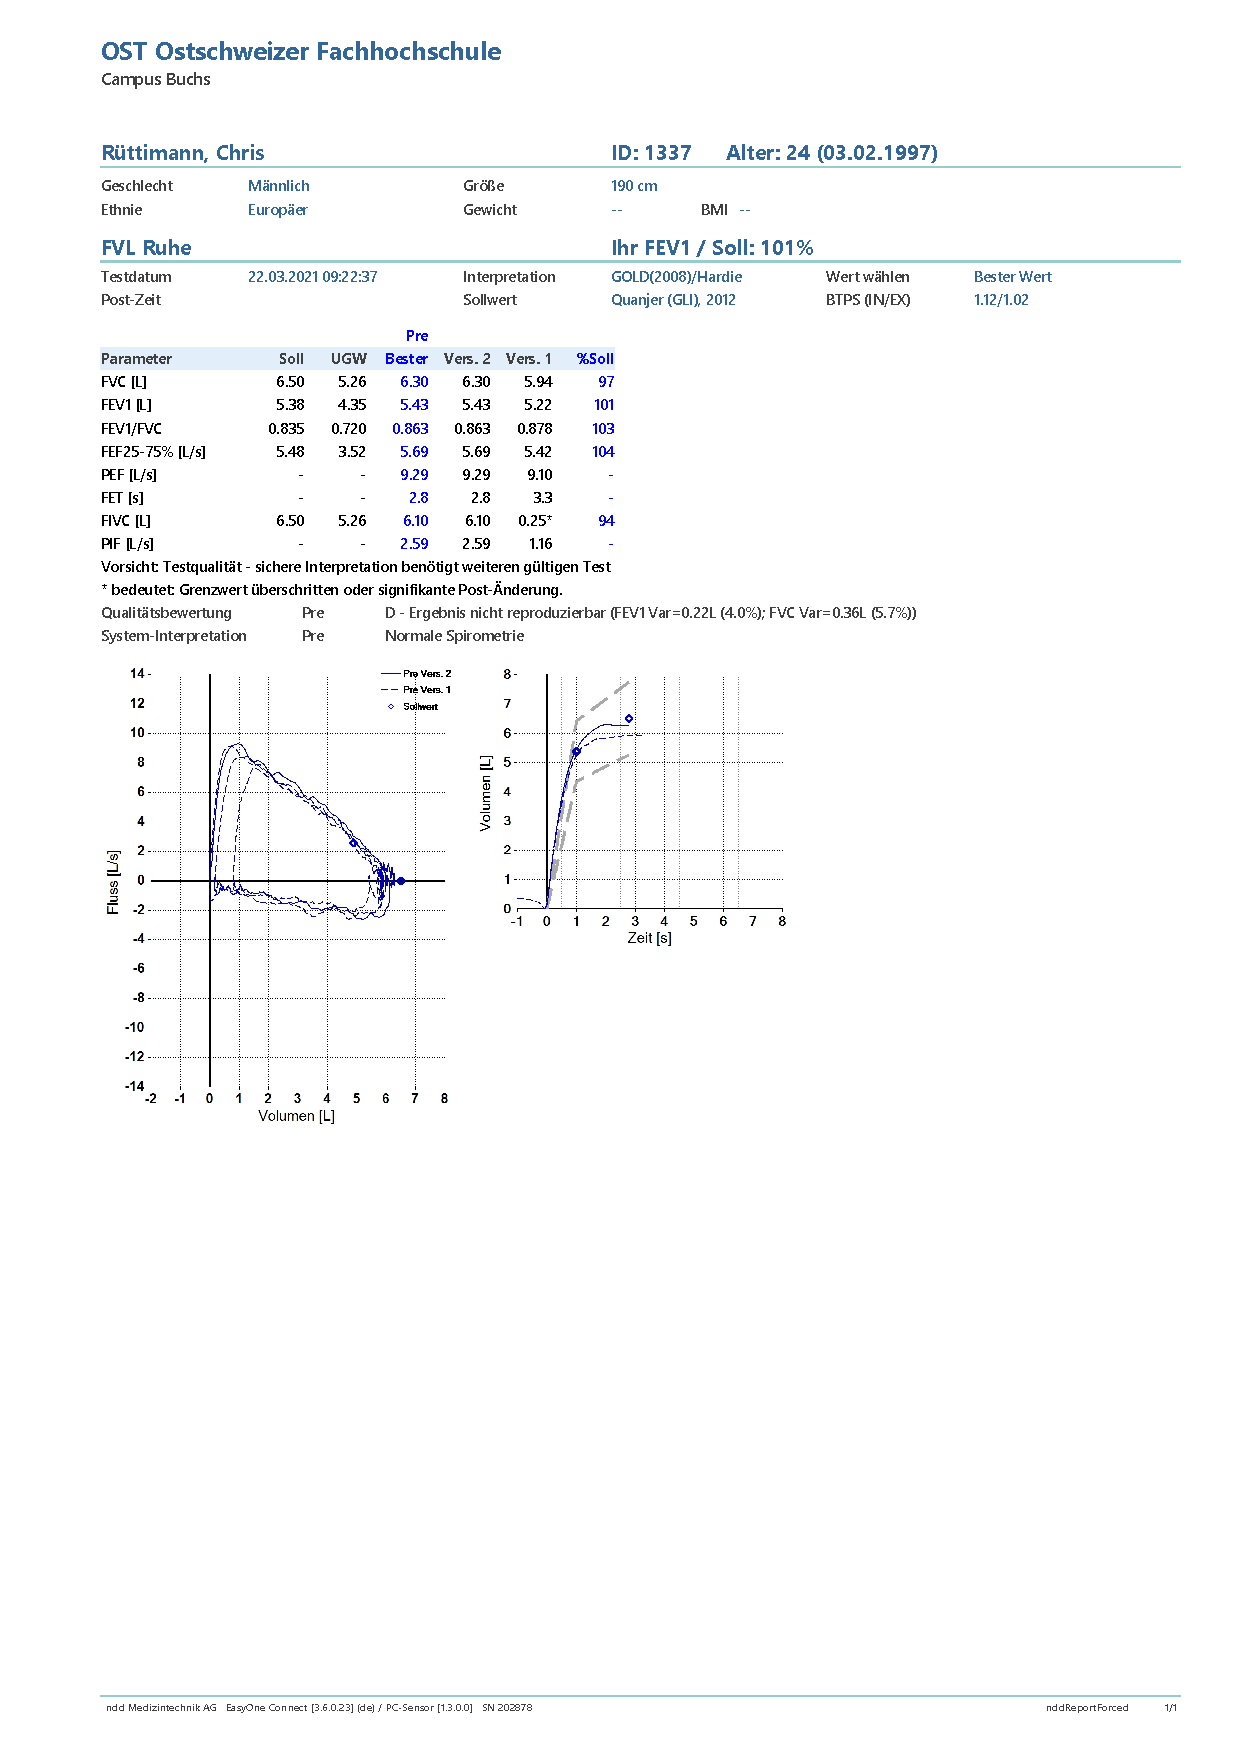
\includegraphics[clip, trim=0cm 10cm 0cm 0cm, width=1.4\textwidth]{Dateien/Chris1.pdf}
    \end{figure}

    \section{Messung 2 Chris}
    \label{sec:chris2}

    \begin{figure}[H]
        \hspace*{-3cm}
        \centering
        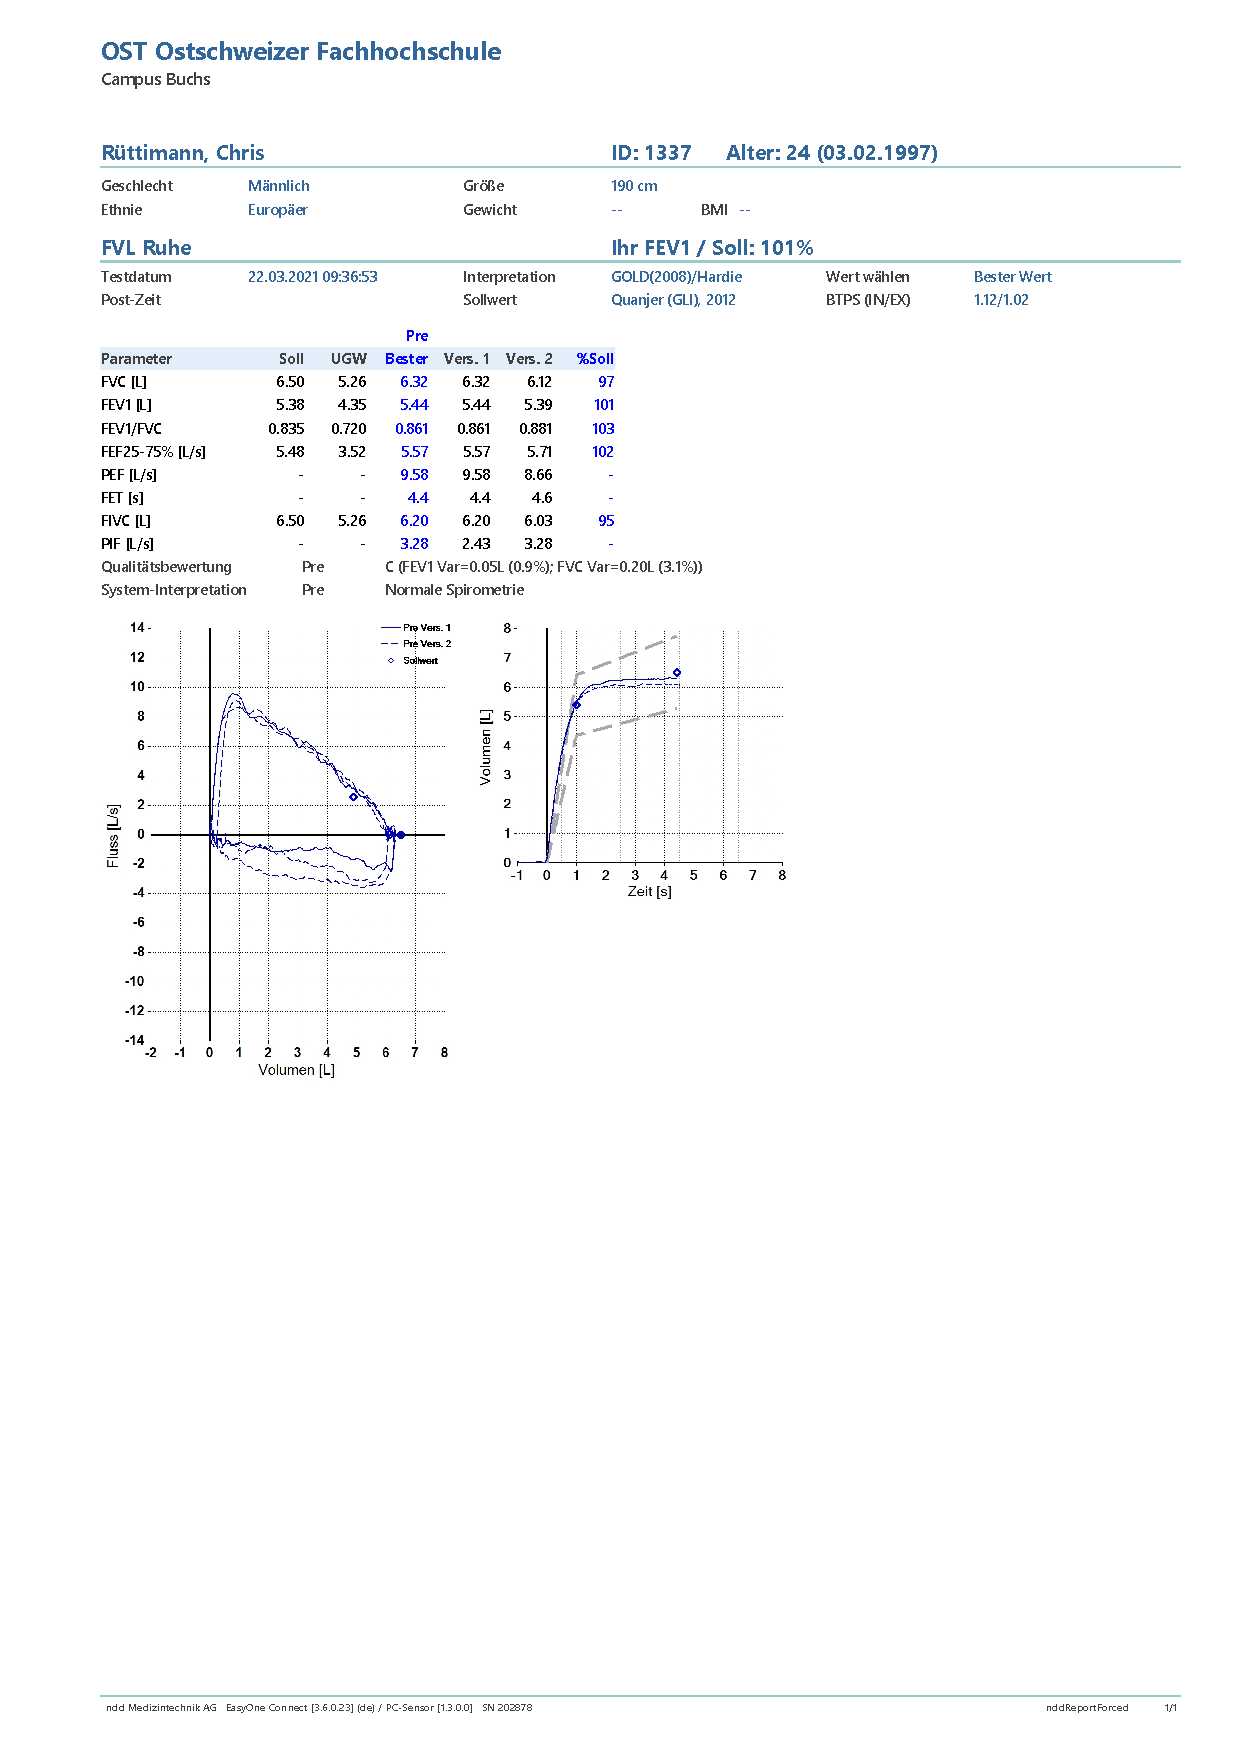
\includegraphics[clip, trim=0cm 10cm 0cm 0cm, width=1.4\textwidth]{Dateien/Chris2.pdf}
    \end{figure}

    \section{Messung 1 Leona}
    \label{sec:leona1}

    \begin{figure}[H]
        \hspace*{-3cm}
        \centering
        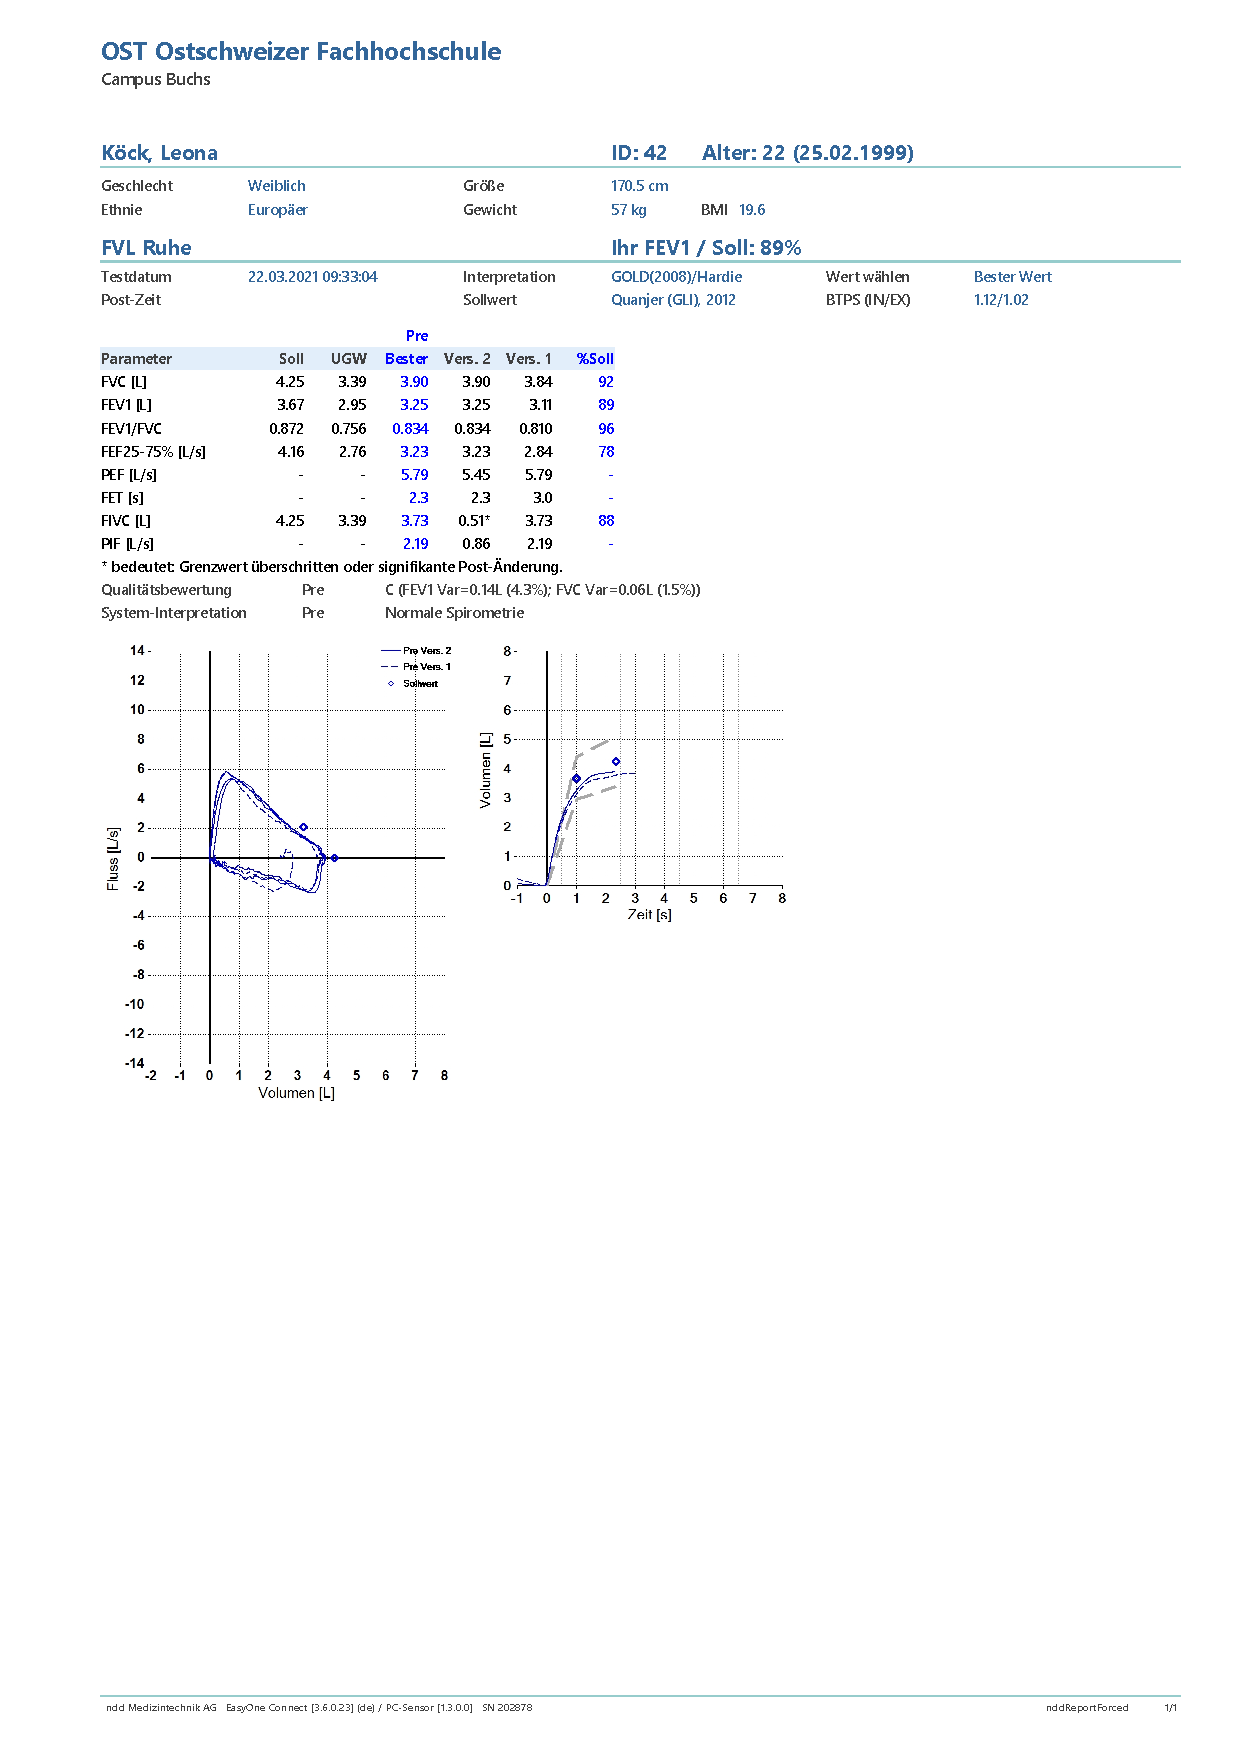
\includegraphics[clip, trim=0cm 10cm 0cm 0cm, width=1.4\textwidth]{Dateien/Leona1.pdf}
    \end{figure}

    \section{Messung 2 Leona}
    \label{sec:leona2}

    \begin{figure}[H]
        \hspace*{-3cm}
        \centering
        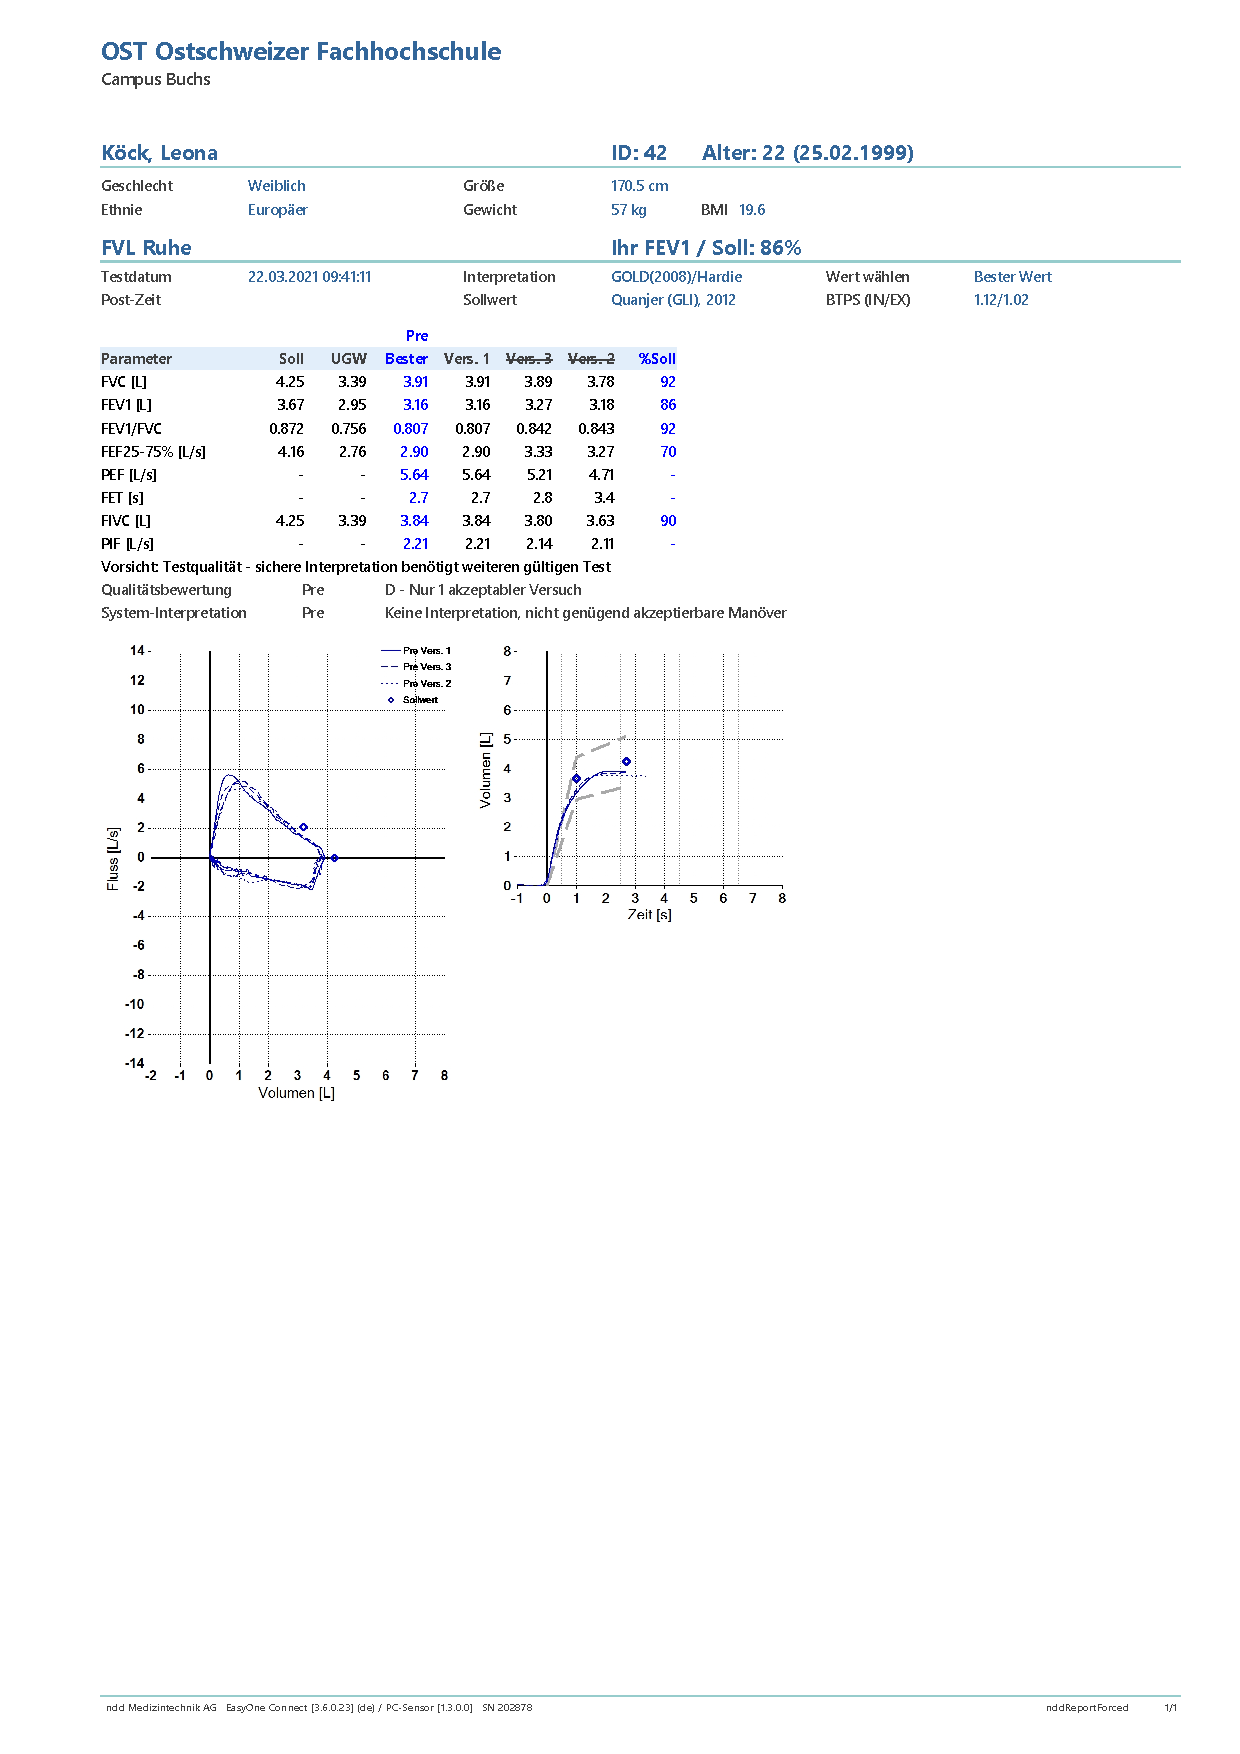
\includegraphics[clip, trim=0cm 10cm 0cm 0cm, width=1.4\textwidth]{Dateien/Leona2.pdf}
    \end{figure}

\end{document}